\chapter{Referencial Teórico}
\label{cap:ref-teorico}

Neste capítulo apresentamos o referencial teórico utilizado neste trabalho. A Seção \ref{ref-teo:pac_rel_ver} discorre sobre \textit{pacote}, \textit{release} e \textit{versão}. A Seção \ref{ref-teo:prov_clie} distingue os termos \textit{provedor} e \textit{cliente}. A Seção \ref{ref-teo:semver} explica o que é \textit{Versionamento Semântico} e o \textit{SemVer} e como eles são utilizados no ecossistema do \textsf{npm}. A Seção \ref{ref-teo:breaking_change} conceitua as \textit{breaking changes} e a Seção \ref{sec:related_works} apresenta os trabalhos relacionados.

\section{Pacote, \textit{Release} e Versão}
\label{ref-teo:pac_rel_ver}
Neste trabalho, o termo \textit{pacote} refere-se a um projeto de \textit{software} hospedado no \textsf{npm}. Cada pacote contêm seu nome, seus arquivos e suas versões. O termo \textit{release} designa o estado de um pacote em um determinado instante. Uma \textit{release} é denotada por um conjunto de arquivos distintos das demais \textit{releases}. O termo \textit{versão} é utilizado para especificar uma \textit{release}. Uma \textit{versão} é uma \textit{string} no padrão do \textit{Versionamento Semântico} onde uma única versão identifica uma única \textit{release} e é utilizada pelo \textsf{npm} no arquivo \textit{package.json}. O arquivo \textit{package.json} é o arquivo de configuração das \textit{releases} que contém todas as informações pertinentes ao pacote naquela \textit{release}, tais como a lista de arquivos, o endereço do repositório, mas principalmente, sua versão única e todos os provedores com as respectivas versões que o cliente aceita. Ainda, o \textit{package.json} contém \textit{scripts} que podem ser executados. Dois deles são os \textit{scripts install} e \textit{test}. Os provedores são instalados por meio do comando \texttt{npm install} e os testes executados através do comando \texttt{npm test}.

\section{Provedor e Cliente}
\label{ref-teo:prov_clie}
\textit{Provedor} é aquele pacote que fornece recursos ao cliente, ou seja, contém interfaces públicas e recursos para acesso às suas funcionalidades. O termo \textit{provedor} também pode ser conhecido como \textit{biblioteca}. Por exemplo, um cliente executa o comando \texttt{npm install mocha}. Após a execução desse comando, o \textsf{npm} registra o \textsf{mocha} no \textit{package.json} como uma dependência. Assim, o pacote \textsf{mocha} é um \textit{provedor direto}, pois foi instalado diretamente pelo cliente. Entretanto, os provedores do \textsf{mocha} também são instalados, mas de forma indireta pelo \textsf{npm}. Estes outros pacotes são chamados de \textit{provedores indiretos} do cliente, pois não dependem que o cliente instale-os manualmente com o comando \texttt{npm install}. A Figura \ref{fig:provider} mostra que o pacote \textsf{mocha} é um provedor direto do \textsf{client}, pois o \textsf{client} requer o \textsf{mocha} para executar. Por sua vez, o pacote \textsf{glob} é um provedor direto do \textsf{mocha} e um provedor indireto do pacote \textsf{client}.

\begin{figure}
    \centering
    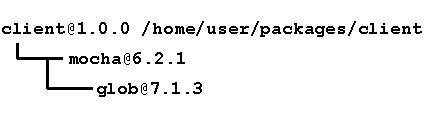
\includegraphics[scale=1.4]{figuras/provider_directly_undirectly.pdf}
    \caption{\textsf{mocha} como provedor direto e \textsf{glob} como indireto do \textsf{client}.}
    \label{fig:provider}
\end{figure}{}

O \textit{cliente} é aquele que está acessando as interfaces públicas do provedor. Quando uma \textit{breaking change} é introduzida pelo provedor -- direto ou indireto --, essa \textit{breaking change} pode se manifestar em qualquer pacote nessa cadeia de dependências, principalmente no cliente. O cliente possui a responsabilidade de atualizar a versão de seus provedores no \textit{package.json} quando esses publicam uma \textit{release} com correções, enquanto o provedor possui a responsabilidade de indicar o nível de compatibilidade que sua nova \textit{release} está introduzindo \cite{teorical_reference:semver}, ou seja, se sua \textit{release} é ou não retro-compatível, através do Versionamento Semântico. O cliente atualiza a versão do seu provedor alterando manualmente essa versão no \textit{package.json} ou instalando outra versão do provedor, fazendo com que o \textsf{npm} atualize a versão no \textit{package.json}. Já o provedor deve conhecer as regras do Versionamento Semântico e cuidar que as suas \textit{releases} sejam versionadas corretamente.

\section{Versionamento Semântico e \textit{SemVer}}
\label{ref-teo:semver}

O Versionamento Semântico\footnote{https://semver.org} é um padrão para versionamento de \textit{releases} de um projeto que considera o tipo de alteração introduzida na \textit{release}. As regras do Versionamento Semântico foram idealizadas por Tom Preston-Werner, criador do \textsf{GitHub}, que incentiva todos os desenvolvedores à utilizarem esse padrão, uma vez que suas regras são baseadas em práticas comuns já utilizadas em projetos \cite{teorical_reference:semver}. Embora sejam apenas um conjunto de regras e não são impostas pelo \textsf{npm}, são largamente utilizadas e incentivadas \cite{decan}. Uma \textit{string} de versão no padrão do Versionamento Semântico possui os níveis \textit{<MAJOR>.<MINOR>.<PATCH>}\footnote{A \textit{string} pode especificar versões \textit{beta, alpha, pre, releases} candidatas, entre outros, tal como \textit{x.y.z-beta.0}} que devem ser incrementados quando o desenvolvedor publicar uma \textit{release}, de acordo com os seguintes critérios:

\begin{itemize}
    \item \textit{MAJOR}: deve ser incrementado quando a \textit{release} introduz \textit{breaking changes}; desobriga a retrocompatibilidade.
    \item \textit{MINOR}: incrementado quando forem adicionadas melhorias/novas funcionalidades que mantenham a compatibilidade com as \textit{releases} anteriores, ou seja, alterações retrocompatíveis; e
    \item \textit{PATCH}: deve ser incrementado quando a \textit{release} contém correção de \textit{bugs}.
\end{itemize}{}

Dessa maneira, se um projeto contém a sua última \textit{release} versionada como \textit{2.1.0}, por exemplo, o seu nível \textit{major} é o 2; o \textit{minor}, 1; e o \textit{patch}, 0. Ao publicar uma nova \textit{release}, se essa contiver uma \textit{breaking change}, então deverá ser publicada com a versão \textit{3.0.0}; se for introduzida uma nova funcionalidade, \textit{2.2.0}; se houver uma correção de \textit{bugs}, \textit{2.1.1}; e se introduzir os três tipos de alterações, o nível \textit{major} deverá ser incrementado, uma vez que uma \textit{breaking change} é a alteração que mais impacta o cliente.

O \textit{SemVer} é uma \textit{string} de versionamento que especifica um intervalo de versões, ou um \textit{range}. Com o \textit{SemVer} é possível especificar quais são as \textit{releases} que o cliente aceita do seu provedor. Há vários padrões de \textit{range}\footnote{https://github.com/npm/node-semver\#ranges} especificados pelo \textit{SemVer}, mas os mais comuns, utilizados pelo \textsf{npm}, são:

\begin{itemize}
    \item \textit{X-Ranges (\textbf{*})}: este \textit{range} especifica para o \textsf{npm} que o cliente aceita qualquer nova \textit{release} do provedor, até mesmo as \textit{releases} com \textit{breaking changes};
    \item \textit{Caret Ranges (\textbf{\textasciicircum})}: este é o \textit{range} mais comum e o padrão do \textsf{npm}. Com o \textit{Caret Range}, o cliente especifica que o \textsf{npm} só deve descarregar novas \textit{releases} do provedor que contenham novas funcionalidades ou/e correções de erros, mas que não contenham \textit{breaking changes}, ou seja, o cliente aceita todas as \textit{releases} das quais foram atualizadas os níveis \textit{patch} ou \textit{minor};
    \item \textit{Tilde Ranges (\textbf{\textasciitilde})}: neste \textit{range}, o cliente especifica para o \textsf{npm} que somente as \textit{releases patch} do provedor são aceitas, ou seja, somente as \textit{releases} que contêm alguma correção de erros.
\end{itemize}{}

O \textsf{npm} utiliza o padrão \textit{SemVer} no arquivo \textit{package.json} pois, através do \textit{SemVer}, o cliente pode decidir o quão flexível ele é ao receber as futuras \textit{releases} dos provedores \cite{decan}. Por exemplo, ao executar o \texttt{npm install express}, para instalar o provedor \textsf{express} por exemplo, o \textsf{npm} -- além de descarregar esse provedor -- irá registrar no \textit{package.json} o nome do provedor com sua versão atual em modo \textit{caret range}, de acordo com a Figura \ref{fig:dep_express}.

\begin{figure}
    \centering
    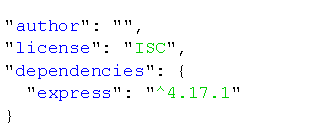
\includegraphics[scale=1.3]{figuras/dependencies_express.pdf}
    \caption{Modo como o \textsf{npm} registra no \textit{package.json} a versão de uma dependência.}
    \label{fig:dep_express}
\end{figure}{}

Com a informação do \textit{range} do provedor no \textit{package.json}, o \textsf{npm} sempre irá resolver o \textit{range} e descarregar as \textit{releases} mais recentes que são aceitas pelo \textit{range SemVer} especificado pelo cliente. \textit{Resolver o range} significa recuperar todas as versões do provedor e selecionar a mais recente que é aceita pela \textit{string SemVer} especificada pelo cliente. Por padrão, o \textsf{npm} especifica o \textit{Caret Range}, mas o cliente pode especificar outro \textit{range} manualmente no \textit{package.json} ou pode utilizar a opção \texttt{--save-exact} junto ao comando \texttt{npm install} para especificar a versão sem o \textit{range}, tornando-se um \textit{range steady}, e fazendo com que o \textsf{npm} sempre instale essa versão específica.

\section{\textit{Breaking Change}}
\label{ref-teo:breaking_change}

Uma \textit{breaking change} é uma alteração no provedor que produz defeitos nos clientes \cite{teorical_reference:semver}. As \textit{breaking changes} surgem quando o provedor, que previamente era executado com sucesso pelo cliente, publica uma \textit{release} que causa um erro ou um comportamento inesperado no cliente. Durante o desenvolvimento de \textit{software}, os provedores precisam introduzir \textit{breaking changes}, pois quando só há \textit{releases} retrocompatíveis, o \textit{software} perde muitas oportunidades de evolução \cite{teorical_reference:bc_2}. Desta maneira, as \textit{breaking changes} são importantes para a evolução de um \textit{software}, e podem ser consideradas sinônimos de evolução. Exemplo disso é o \textsf{Node.js}, que publica uma \textit{release} incrementando o nível \textit{major} a cada 6 meses.\footnote{https://github.com/nodejs/node\#release-types} Introduzir \textit{breaking changes} em níveis \textit{major} permite que os \textit{softwares} evoluam sem manter-se presos à versões anteriores.

Para evitar que os impactos de uma \textit{breaking change} afetem os clientes, os provedores devem publicar suas \textit{releases} com \textit{breaking changes} sempre incrementando o nível \textit{major} da sua nova versão, seguindo as regras do Versionamento Semântico. Dessa maneira, os clientes de versões prévias que especificaram os provedores com o \textit{range caret} -- \textit{range} especificado por padrão pelo \textsf{npm} -- ou o \textit{range tilde}, não são afetados por uma \textit{breaking change}, pois eles apenas aceitam \textit{releases} com novas funcionalidades e correções de erros -- \textit{releases minor} e \textit{patch}, respectivamente. Entretanto, uma \textit{breaking change} pode ser introduzida erroneamente quando são atualizados os níveis \textit{minor} ou \textit{patch}. Dessa maneira, o problema das \textit{breaking changes} está no fato dos provedores introduzirem em \textit{releases minor} ou \textit{patch}, o que não é esperado pelos clientes, resultando em defeitos nos clientes.

% \subsection{\textit{Breaking without-change}}
\subsection{\textit{Breaking change} induzida}
\label{subsec:break_without}
Além de alterações que resultam em \textit{breaking changes}, há algumas alterações que são geradas nos provedores mas que, nessa pesquisa, não serão consideradas como \textit{breaking changes}, uma vez que esses casos não significam que o provedor contenha um erro ou não fazem parte do ecossistema do \textsf{npm}. Os erros do tipo \textit{breaking change induzido} são erros que não são gerados por uma nova \textit{release} do provedor e nem podem ser corrigidas em uma próxima \textit{release} do provedor. Essas alterações são:

\begin{itemize}
    % \item Dois pacotes que requerem versões específicas e distintas do \textsf{Node.js}: o \textsf{Node.js} atualizou o seu nível \textit{major} de \textit{0.x} para \textit{7.x} em apenas 3 anos,\footnote{https://nodejs.org/en/download/releases} mas isso não significa que os pacotes evoluíram seus códigos sempre para a última \textit{release} do \textsf{Node.js}, e o inverso é valido, ou seja, os pacotes podem ter evoluído seus códigos na mesma frequência do \textsf{Node.js}. Por exemplo, considere um cliente executando no \textsf{Node.js} \textit{0.x} com um provedor que evoluiu seu código para a sintaxe do \textsf{Node.js} \textit{6.x}, que não é aceita no \textsf{Node.js} \textit{0.x}. Desta maneira, não há uma versão do \textsf{Node.js} na qual seja possível executar o cliente e o provedor sem que seja manifestado um erro por causa do \textsf{Node.js}. Assim, erros nos provedores ocasionados por versões do \textsf{Node.js} não serão considerados como \textit{breaking changes}, pois o erro é causado pelo \textsf{Node.js}, que não reconhece a sintaxe, e não pelo provedor;

    \item Exclusão de uma \textit{release}/\textit{provedor} do \textsf{npm}: pelas regras do \textsf{npm}, uma \textit{release} só pode ser removida até 72 horas após ter sido publicada.\footnote{https://docs.npmjs.com/cli/unpublish\#description} Entretanto, quando uma \textit{release} é removida do \textsf{npm} e o cliente especificou aquela \textit{release}, isso gera um erro no \textit{script install}. Assim, o erro é causado pelo \textsf{npm} que não consegue encontrar a \textit{release}, e não pelo provedor. No caso do provedor ter sido removido do \textsf{npm} a situação é a mesma: um provedor só pode ser removido após 72 horas. Entretanto, anterior ao acontecimento do \textsf{left-pad}, os pacotes -- e \textit{releases} também -- podiam ser removidos do \textsf{npm} em qualquer circunstância. Por isso, quando um erro foi causado pela falta de um pacote que foi removido do \textsf{npm}, não foi considerado como uma \textit{breaking change};

    \item Alterações em serviços externos: os provedores podem fazer uso de sistemas externos, tais como acesso à \textit{APIs} de sites e sistemas, e recuperar dados. Entretanto, ao longo do tempo, naturalmente, essas \textit{APIs} podem alterar seus dados, o que gera inconsistências em seus clientes. Mas esse tipo de erro não é considerado como uma \textit{breaking change}, uma vez que esse caso não faz parte do ecossistema do \textsf{npm} e o provedor não tem controle sobre esses dados.
    % ACTUALLY, THE NEXT EXAMPLE IS JUST A NORMAL CASE OF ERROR THAT I CONSIDERED AS A NORMAL
    %\item Cliente aceita \textit{releases major} do provedor: quando o cliente especifica em seu \textit{package.json} que aceita qualquer \textit{release} do provedor, através de um \textit{X-range}, o cliente então também está aceitando \textit{releases} que introduziram \textit{breaking changes}. Por isso, quando um cliente for impactado por uma \textit{breaking change} no provedor, e que foi corretamente introduzida em uma \textit{release major}, significa que o problema está no cliente que aceitou a \textit{breaking change} mas não a tratou.
\end{itemize}{}

\section{Trabalhos Relacionados}
\label{sec:related_works}
Esta Seção apresenta os trabalhos relacionados ao tema \textit{breaking change}. Na Subseção \ref{sub:related:npm} estão os trabalhos relacionados a estudos no ecossistema do \textsf{npm}. A Subseção \ref{sub:related:others} descreve os trabalhos sobre \textit{breaking changes} em outros ecossistemas.

\subsection{\textit{Breaking changes} no \textsf{npm}}
\label{sub:related:npm}

\citeonline{teorical_reference:bc_2} apresentam um estudo sobre a estabilidade das dependências no ecossistema do \textsf{npm} e do \textsf{CRAN}. Os autores entrevistaram setes mantenedores de pacotes e questionaram os entrevistados sobre os motivas das mudanças em seus \textit{softwares}. Os desenvolvedores afirmaram que o Versionamento Semântico deve ser usado corretamente para evitar problemas com atualizações de dependências. Em nosso trabalho, descobrimos que os provedores realmente introduzem e publicam alterações em níveis incorretos do Versionamento Semântico. Essas publicações, usando um versionamento incorreto, realmente introduzem erros nos pacotes clientes, encerrando a execução.

O trabalho de \citeonline{teorical_reference:bc_1} apresenta uma abordagem para detectar \textit{breaking changes} em \textit{APIs} em três pacotes provedores. O autor selecionou \textit{1k} pacotes clientes para cada pacote provedor e realizou um \textit{parser} nos códigos dos clientes e dos provedores. Assim, foi possível descobrir, entre duas versões de um provedor, se houve alteração em uma de suas \textit{APIs}. O \textit{parser} no código do cliente foi realizado para verificar se algum cliente utilizava alguma \textit{API} do provedor que havia sido alterada. Ao todo, foram identificados de 9.8\% a 25.8\% de \textit{releases} dos clientes haviam sido impactadas com alguma \textit{breaking change} nas \textit{APIs} dos provedores. Em nosso trabalho nós identificamos que 13.9\% de \textit{releases} dos pacotes clientes foram impactadas por algum tipo de \textit{breaking change}. Porém, o método do autor é melhor do que o nosso para identificar \textit{breaking changes} em \textit{APIs}, uma vez que, em nosso trabalho, alterações nos argumentos de \textit{APIs} podem não ter sido detectadas (Ver Seção \ref{cap:threats}).

\citeonline{noregrets2018} apresentam uma técnica chamada \textit{teste de regressão de tipo} para verificar alteração no tipo dos objetos retornados de uma \textit{API}. Essa técnica consiste em executar uma chamada para uma \textit{API}, salvar o tipo do objeto retornado, executar novamente a \textit{API}, salvar o tipo do objeto retornado nessa última execução e comparar ambos os tipos. A \textit{release} do provedor é alterada entre as duas execuções para verificar se o tipo do objeto foi alterado entre as duas \textit{releases} do provedor. Os autores escolheram os 12 provedores mais populares do \textsf{npm} para realizar as análises. Para todas as versões \textit{major} de um provedor, foi executado as \textit{APIs} de todas as \textit{releases minor} e \textit{patch} pertencentes àquela versão \textit{major}. Então foi aplicada o teste de regressão nessas versões \textit{minor} e \textit{patch}. Foi constatado regressão no tipo dos objetos em 9.4\% das \textit{releases}. Nosso trabalho aborda qualquer tipo de \textit{breaking changes} e nossa análise é tanto no pacote cliente quanto no pacote provedor, com um total de 13.9\% de \textit{releases} dos clientes afetadas com \textit{breaking changes}.

O trabalho de \citeonline{using_others_tests} foca na detecção de \textit{releases} de provedores que induzem um erro na execução dos clientes. Os autores analisaram um total de \textit{290k} pacotes do \textsf{npm}. Eles verificaram nos repositórios dos clientes todos os \textit{commits} que alteraram o \textit{package.json}. Para os provedores especificados com versões \textit{range}, foi resolvido a versão do provedor com base na data do \textit{commit}. Entre dois \textit{commits}, os autores verificaram se a versão do provedor foi retrocedida, ou seja, se foi realizado um \textit{downgrade}. Quando houve o \textit{downgrade}, a versão atual e a prévia do provedor foi registrada como uma possível \textit{release} com \textit{breaking change}. Ou seja, se o pacote cliente realizou um \textit{downgrade}, pode ter sido realizado por causa de uma \textit{breaking change}. Finalmente, dez casos aleatórios de \textit{downgrade} foram selecionados e os testes dos clientes foram executados com a \textit{release} atual e a prévia do provedor e foi verificado se houve um erro na execução do cliente entre a versão atual e prévia. Foi observado um total de 4.1\% das \textit{releases} dos clientes falharam após a atualização do provedor. Nossa metodologia não analisou a cobertura dos testes dos clientes, enquanto que os autores a fizeram. Como os autores, usamos dados oriundos do \textsf{npm} e resolvemos as versões dos provedores, mas nós executamos os testes dos clientes sempre que pelo menos uma versão dos provedores foi alterada.

\subsection{\textit{Breaking changes} em outros ecossistemas}
\label{sub:related:others}
\citeonline{whyandhowluceneremovethiswords} estudaram 400 provedores no repositório do \textsf{Maven} por um total de 116 dias. Os pacotes provedores foram escolhidos pela popularidade medida no \textsf{GitHub} e, durante aquele período, os autores analisaram os \textit{commits} que introduziram uma \textit{breaking change} em uma \textit{API}. Quando uma \textit{breaking change} em algum \textit{commit} foi detectada, eles questionaram o autor do \textit{commit} sobre o motivo para introduzir aquela \textit{breaking change}. Os autores observaram que 33.3\% das \textit{breaking changes} são inseridas para implementar novas funcionalidades e 29.8\% para simplificar as \textit{APIs}. Em nosso trabalho nós focamos em encontrar as \textit{breaking changes} através dos testes dos pacotes clientes e nós encontramos que o tipo mais comum de \textit{breaking changes} são as \textit{Alterações de uma funcionalidade}, que foi introduzida em 39.06\% dos casos.

O trabalho de \citeonline{Foo:2018:ESC:3236024.3275535} apresenta um estudo sobre \textit{breaking changes} em \textit{APIs} nos ecossistemas \textsf{Maven}, \textsf{PyPI} e \textsf{RubyGems}. O objetivo do trabalho de \citeonline{Foo:2018:ESC:3236024.3275535} é analisar uma ferramenta desenvolvida para esse propósito, que realiza automaticamente uma análise estática e eficiente para verificar se a atualização para uma versão de um provedor introduz uma \textit{breaking change} de \textit{API}. A ferramenta detecta \textit{breaking changes} computando um \textit{diff} entre o código de duas \textit{releases} de um pacote provedor. Foram descobertas \textit{breaking changes} em 26\% dos pacotes provedores e a ferramenta conseguiu sugerir atualizações automaticamente para 10\% dos pacotes. Nosso método vai além de descobrir \textit{breaking changes} apenas em \textit{APIs} e concluímos que 11.7\% dos pacotes clientes são impactados por \textit{breaking changes}.